
\chapter{Reconstruction of the Multilayer Structure by Specular Measurement Methods} \label{ch_spec}
The multilayer mirror samples we shall investigate here were fabricated using the magnetron sputtering technique briefly discussed in the chapter~\ref{ch_exp} with nominal layer thicknesses and chemical species, depending on the desired reflection angle and spectral range. Among other parameters of the production process, the achieved layer thickness and sharpness of the interfaces has a direct impact on the performance of these mirrors with respect to their peak reflectance and bandwidth. Although the sputtering process is a well established technique for mirror fabrication, the actual layer thicknesses in the sample may differ from the nominal values and are generally unknown.

Based on the matrix algorithm introduced in chapter~\ref{ch_theo}, the electromagnetic fields   inside and outside an arbitrary layer system can be calculated. Most importantly, this allows to calculate the expected specular reflectance curves across angular or spectral ranges for a given layer model. The comparison of these calculated curves to measured data thus allows to obtain information about the actual layer properties in a given sample. However, the detected reflectance values in a specular reflection experiment are merely intensities of reflected radiation. The information on the phase of the electromagnetic wave can not be obtained in this way and is lost. It is thus not possible to directly reconstruct the layout of the sample with the measured reflection curve. This is known as the inverse problem of scatterometry. Reconstructing the layer properties is therefore an attempt of solving this inverse problem by accumulating prior knowledge about the sample, such as the nominal design goals during the fabrication process, into a model of that system. Starting from this model, the theoretically calculated curve is compared to the measured reflectance and optimized iteratively.

\begin{itemize}
 \item more about what people already do
 \item what are the problems (no unique solution)
 \item solution approach: PSO
 \item test
 \item validation with MCMC and confidence intervals
 \item combination of several methods to improve
 \item for Cr/Sc: standard model does not work anymore, better model necessary
 \item for Cr/Sc: how can better model be solved uniquely?
\end{itemize}


This method is not limited to the optimization of the model with respect to the reflectance of the mirror samples in their designated \gls{euv} spectral range. In order to add complementary information for refining the solution of the inverse problem, additional methods can be applied. In this chapter, depending on the sample system, we analyze several experimental methods. Apart from the aforementioned reflectance in the \gls{euv} spectral range, we apply resonant \gls{euv} reflectance across absorption edges, \gls{xrr} with high photon energy and finally \gls{xrf}. The latter does rely on the measurement of fluorescence radiation and thus requires the calculation of the field intensities inside the layer stack at the position of a specific chemical species for its analysis as described in section~\ref{ch_theo:sec_xrf} of chapter~\ref{ch_theo}.

This chapter consists of three parts attributed to the study of three sample system categories. Firstly, the analysis of the specular \gls{euv} reflectance is applied and discussed in detail in section~\ref{ch_spec:sec_reconstruction_PTB17} to a high-reflectance multilayer mirror composed out of Mo/B$_4$C/Si/C optimized for reflection in the spectral range between $\lambda=\nm{12.4}$ and $\lambda=\nm{14.0}$ at angles of incidence below $\alpha_i \leq \SI{15}{\degree}$ based on the data at those wavelengths and angles.

Secondly, a system 


\section{Reconstruction Based on Specular EUV reflectance} \label{ch_spec:sec_reconstruction_PTB17}
\begin{figure}[htbp]
\centering
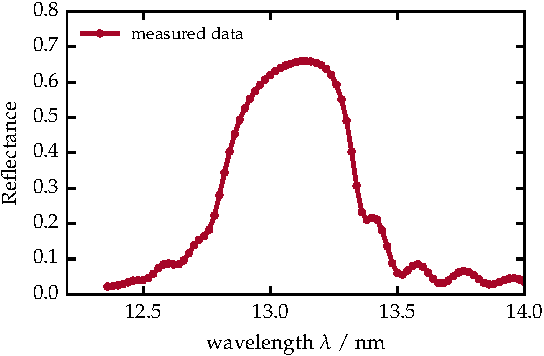
\includegraphics{img/PTB17_reflectance_AOI_15}
\caption{Specrally resolved reflectance data of the Mo/B$_4$C/Si/C multilayer sample. The irradiation was conduced under a fixed angle of incidence $\alpha_i = 15.0^\circ$. The measurement uncertainty is within the line thickness of the plot.}
\label{ch_spec:fig_ptb17_reflectance_AOI_15}
\end{figure}

\cite{haase_role_2014}



\subsection{Multilayer Model and Particle Swarm Optimization}
\gls{pso}
\begin{figure}[htbp]
    \def\svgwidth{0.7\textwidth}
    \fontfamily{fds}\selectfont\footnotesize
    \import{svg/}{mo_si_ptb17_model.pdf_tex}
    \caption{Model of the multilayer stack including the substrate and the capping layers. The periodic part is enclosed between the dashed lines with four layers in each period repeated $N=64$ times. The capping period does not include an interdiffusion layer but has a natural SiO$_2$ layer.}
    \label{fig:model}
\end{figure}

\begin{table*}
\centering
\caption{Multilayer parametrization and parameter limits}
\label{tbl:multilayer_parameters}
\begin{tabular}{@{}llll@{}}
\toprule
Parameter & Definition & Lower bound & Upper bound\\ \midrule
$d_\text{Mo}$ / nm & Mo layer thickness & $0.0$& $7.0$\\ 
$d_\text{Si}$ / nm & Si layer thickness& $0.0$& $7.0$\\ 
$d_\text{C}$ / nm &C buffer layer thickness& $0.0$ & $5.0$\\ 
$d_\text{B$_4$C}$ / nm &B$_4$C buffer layer thickness&$0.0$ & $5.0$\\ 
$\sigma$ / nm & N\'{e}vot-Croce parameter& $0.0$& $2.0$\\ 
&(identical for all interfaces)&&\\
$\rho_\text{Mo}$ &Mo density w.r.t.~bulk density & $0.5$& $1.0$\\ 
$\rho_\text{Si}$ &Si density w.r.t.~bulk density& $0.5$& $1.0$\\ 
$\rho_\text{C}$ &C density w.r.t.~bulk density& $0.5$& $1.0$\\ 
$\rho_\text{B$_4$C}$ &B$_4$C density w.r.t.~bulk density& $0.5$& $1.0$\\
\midrule
\multicolumn{4}{c}{Capping layer}\\
\midrule
$d_\text{SiO$_2$(cap)}$ / nm & SiO$_2$ capping layer thickness & $0.0$&$5.0$ \\ 
$\rho_\text{SiO$_2$(cap)}$& $=\rho_\text{Si}$ (identical to Si density)& & \\
 \bottomrule
\end{tabular}
\end{table*}

\begin{figure}[htbp]
\centering
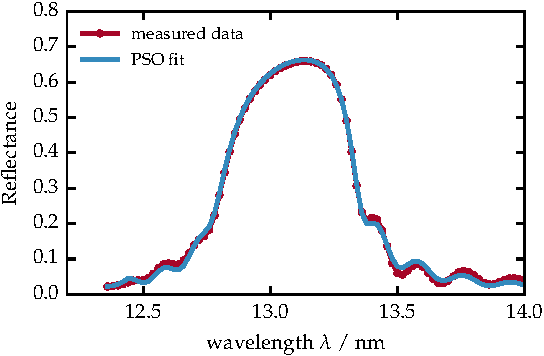
\includegraphics{img/PTB17_reflectance_AOI_15_fitted}
\caption{Theoretical reflectance curve based on the optimal model parameters obtained from the particle swarm optimization.}
\label{ch_spec:fig_ptb17_reflectance_AOI_15_fitted}
\end{figure}

\subsection{The Problem of Model Uniqueness}
\begin{figure*}[htbp]
\centering
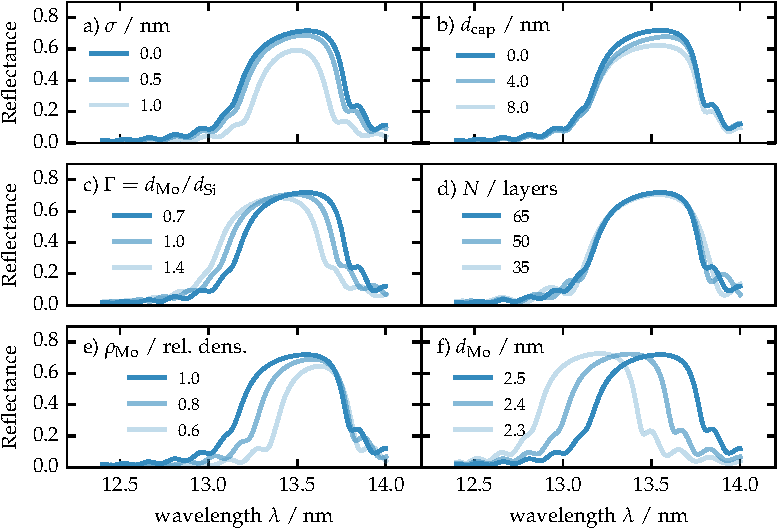
\includegraphics{img/parameter_influence}
\caption{Parameter influence.}
\label{ch_spec:fig_mo_si_parameter_influence}
\end{figure*}

\subsection{Markov-chain Monte Carlo Verification}
MCMC use with multilayers: \cite{hobson_markov-chain_2004}
\begin{figure*}[htbp]
\centering
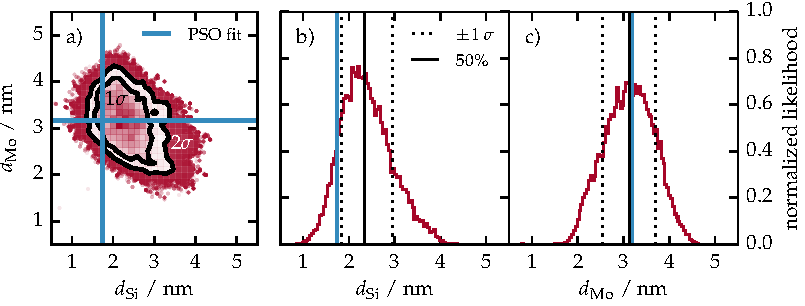
\includegraphics{img/PTB17_MCMC_d_Mo_vs_d_Si}
\caption{Specrally resolved reflectance data of the Mo/B$_4$C/Si/C multilayer sample. The irradiation was conduced under a fixed angle of incidence $\alpha_i = 15.0^\circ$. The measurement uncertainty is within the line thickness of the plot.}
\label{ch_spec:fig_ptb17_MCMC_d_Mo_vs_d_Si}
\end{figure*}

\begin{figure*}[htbp]
\centering
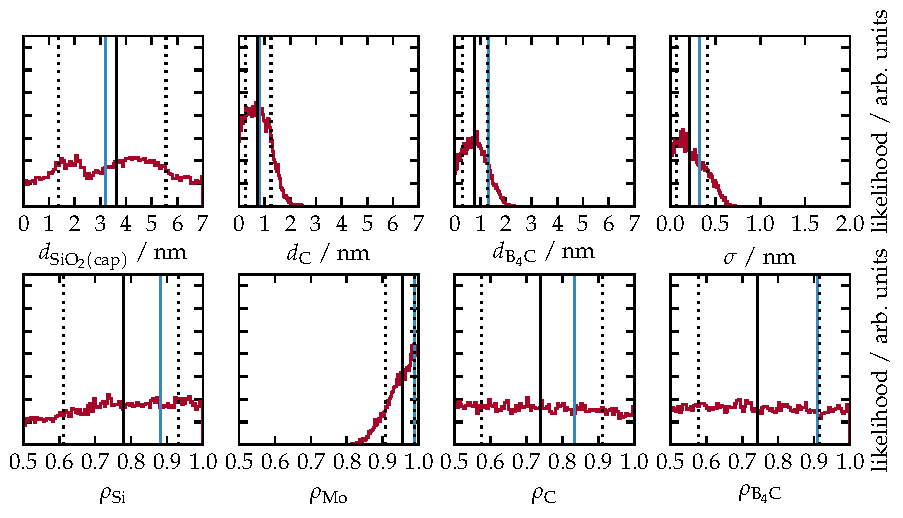
\includegraphics{img/PTB17_MCMC_other_params}
\caption{Specrally resolved reflectance data of the Mo/B$_4$C/Si/C multilayer sample. The irradiation was conduced under a fixed angle of incidence $\alpha_i = 15.0^\circ$. The measurement uncertainty is within the line thickness of the plot.}
\label{ch_spec:fig_ptb17_MCMC_other_params}
\end{figure*}



\section{Molybdenum Thickness Variation in Mo/Si Multilayers}

\subsection{Combined Analysis of X-ray and EUV reflectance}
The reconstruction of the model for the multilayer itself as well as of the power spectral density for the interfacial roughness is an optimization problem. Based on the measured reflectivity data and the diffuse scattering, respectively, in each case, an optimization functional defines the goodness of the model. The optimization functional can then be described for each of the methods (EUV, XRR, diffuse scattering) individually by the reduced $\tilde{\chi}^2$
\begin{align}
\tilde{\chi}^2 = \frac{1}{m - p} \bigg[\sum\limits_{m} \frac{(I_m^\text{model} 
- I_m^\text{meas})^2}{\tilde{\sigma}_m^2} \bigg] \text{,} 
\label{eqn:reduced_chi_2}
\end{align}
where $m$ is the number of measurement points, $p$ is the number of parameters used in the model, $I_m^\text{model}$ is the calculated intensity for the corresponding measurement point with index $m$ having the measured intensity $I_m^\text{measured}$. The calculated intensity $I_m^\text{model}$ follows directly from $R$ in Eq.~\eqref{eqn:refl_trans} for the EUV and XRR measurements and $\big(d \sigma/d \Omega\big)$ in Eq.~\eqref{eqn:dwba} for the diffuse scattering, respectively, in each case, for the angle of incidence and wavelength associated with measurement point $m$. The experimental error for each measurement point is described by $\tilde{\sigma}_m$. The combined functional for the analysis of the EUV and X-ray reflectance experiments to be optimized with respect to the measured data is defined as
\begin{align}
\chi^2 = \tilde{\chi}^2_\text{EUV} +\tilde{\chi}^2_\text{XRR} \text{,}
\label{eqn:total_chi_2}
\end{align}
and for the diffuse scattering as
\begin{align}
\chi^2 = \tilde{\chi}^2_\text{diff} \text{.} \label{eqn:total_chi_2_diffuse}
\end{align}
The solution to the inverse problem of reconstructing the optimal model parameters is conducted by minimizing the $\chi^2$ functional. To minimize the functional with respect to the best choice of parameters, we apply a Markov-chain Monte Carlo method \cite{goodman_ensemble_2010,foreman-mackey_emcee:_2013,haase_multiparameter_2016}. As a starting point, a random set of parameters is generated with respect to predefined boundaries. The limits are chosen in reference to prior knowledge and physical plausibility. The advantage of this procedure with respect to other optimization methods such as Levenberg-Marquart \cite{levenberg_method_1944,marquardt_algorithm_1963} or particle swarm optimization \cite{kennedy_particle_2011} is that the distribution of the Monte Carlo walkers after convergence reflects the set of parameters with maximum likelihood, correlations in between the parameters as well as confidence intervals for each value within the underlying model. The latter ones are estimated from the MCMC as one standard deviation of the sample distribution in each parameter.

\subsection{Reconstruction of the Mo Layer Thickness}
\paragraph{Model of the Multilayer Stack} \label{sec:mo_si_model}
The thicknesses of the Mo layers inside the stack were varied nominally from $1.7$ nm to $3.05$ nm from sample to sample. The stacking of the different layers in the multilayer consists of the Mo and Si layers, as well as an additional buffer layer at the Si-to-Mo interface to prevent interdiffusion. For the Mo-to-Si interfaces, no buffer layers were included since interdiffusion is usually less in this case \cite{petford-long_highresolution_1987}. However, for the theoretical description of the sample stack we consider an additional MoSi$_2$ layer, which is well known to form during the deposition process \cite{bajt_investigation_2001}. The full model used in the reconstruction is illustrated in Fig.~\ref{fig:model} with the thickness parameters for each layer. To correct for any contamination on the top sample surface, an additional carbon-like layer on top was considered. In addition to the thicknesses of each layer we also allowed for a variation of the layer density between $80\%$ and $100\%$ of the bulk density. The evaluation of the reflectivity with respect to the model was performed with the matrix algorithm in Eq.~\eqref{eqn:refl_trans} described above. The model parameters and their boundaries are listed in Table~\ref{tbl:multilayer_parameters}.
\begin{figure}[htbp]
    \def\svgwidth{0.7\textwidth}
    \fontfamily{fds}\selectfont\footnotesize
    \import{svg/}{mo_si_iws_model.pdf_tex}
    \caption{Model of the multilayer stack including the substrate and the capping layers. The periodic part is enclosed between the dashed lines with four layers in each period repeated 49 times. The capping period does not include an interdiffusion layer but has a natural SiO$_2$ layer and a carbon-like layer accounting for contamination on the top surface.}
    \label{fig:model}
\end{figure}
\begin{table*}
\centering
\caption{Multilayer parametrization and parameter limits}
\label{tbl:multilayer_parameters}
\begin{tabular}{@{}llll@{}}
\toprule
Parameter & Definition & Lower bound & Upper bound\\ \midrule
$d_\text{Mo}$ / nm & Mo layer thickness & $0.0$& $4.5$\\ 
$d_\text{Si}$ / nm & Si layer thickness& $0.0$& $7.0$\\ 
$d_\text{C}$ / nm &C buffer layer thickness& $0.0$ & $0.6$\\ 
$d_\text{MoSi$_2$}$ / nm &MoSi$_2$ interdiffusion layer thickness&$0.0$ & $0.6$\\ 
$\sigma$ / nm & N\'{e}vot-Croce parameter& $0.0$& $0.5$\\ 
&(identical for all interfaces)&&\\
$\rho_\text{Mo}$ &Mo density w.r.t.~bulk density & $0.8$& $1.0$\\ 
$\rho_\text{Si}$ &Si density w.r.t.~bulk density& $0.8$& $1.0$\\ 
$\rho_\text{C}$ &C density w.r.t.~bulk density& $0.8$& $1.0$\\ 
$\rho_\text{MoSi$_2$}$ &MoSi$_2$ density w.r.t.~bulk density& $0.8$& $1.0$\\
\midrule
\multicolumn{4}{c}{Capping layer}\\
\midrule
$d_\text{C(cap)}$ / nm & C capping layer thickness & $0.0$&$3.0$ \\ 
$d_\text{SiO$_2$(cap)}$ / nm & SiO$_2$ capping layer thickness & $0.0$&$1.5$ \\ 
$\rho_\text{C(cap)}$ &C capping layer density w.r.t.~bulk density& $0.0$& $1.0$\\ 
$\rho_\text{SiO$_2$(cap)}$& $=\rho_\text{Si}$ (identical to Si density)& & \\
 \bottomrule
\end{tabular}
\end{table*}

%In order to obtain a unique reconstruction of the multilayer stack thicknesses and densities, a combination of several methods is necessary \cite{}\todo{citation Cr/Sc paper}. This is in general a very time consuming procedure, since many complementary methods have to be applied for all samples. In case of the sample system of interest here, the samples ideally only differ in the thickness of the Mo layers. We therefore focus on the unambiguous determination of the corresponding thicknesses here. In this case the combined analysis of EUV reflectivity and X-ray reflectivity suffice.

\paragraph{Specular Measurement Results and Optimization} \label{sec:mo_si_model_reconstruction_results}
The two sample sets have been measured with respect to their reflectivity at a fixed angle of incidence $\alpha_i=15^\circ$ from the surface normal by varying the wavelength in the spectral range from $\lambda=12.4$ nm to $\lambda=14.0$ nm. The results are shown in Fig.~\ref{fig:EUV_reflectivity} in comparison to each other, with their nominal Mo layer thickness. The max.~peak reflectance is also shown for the two series.
\begin{figure*}[htbp]
\centering
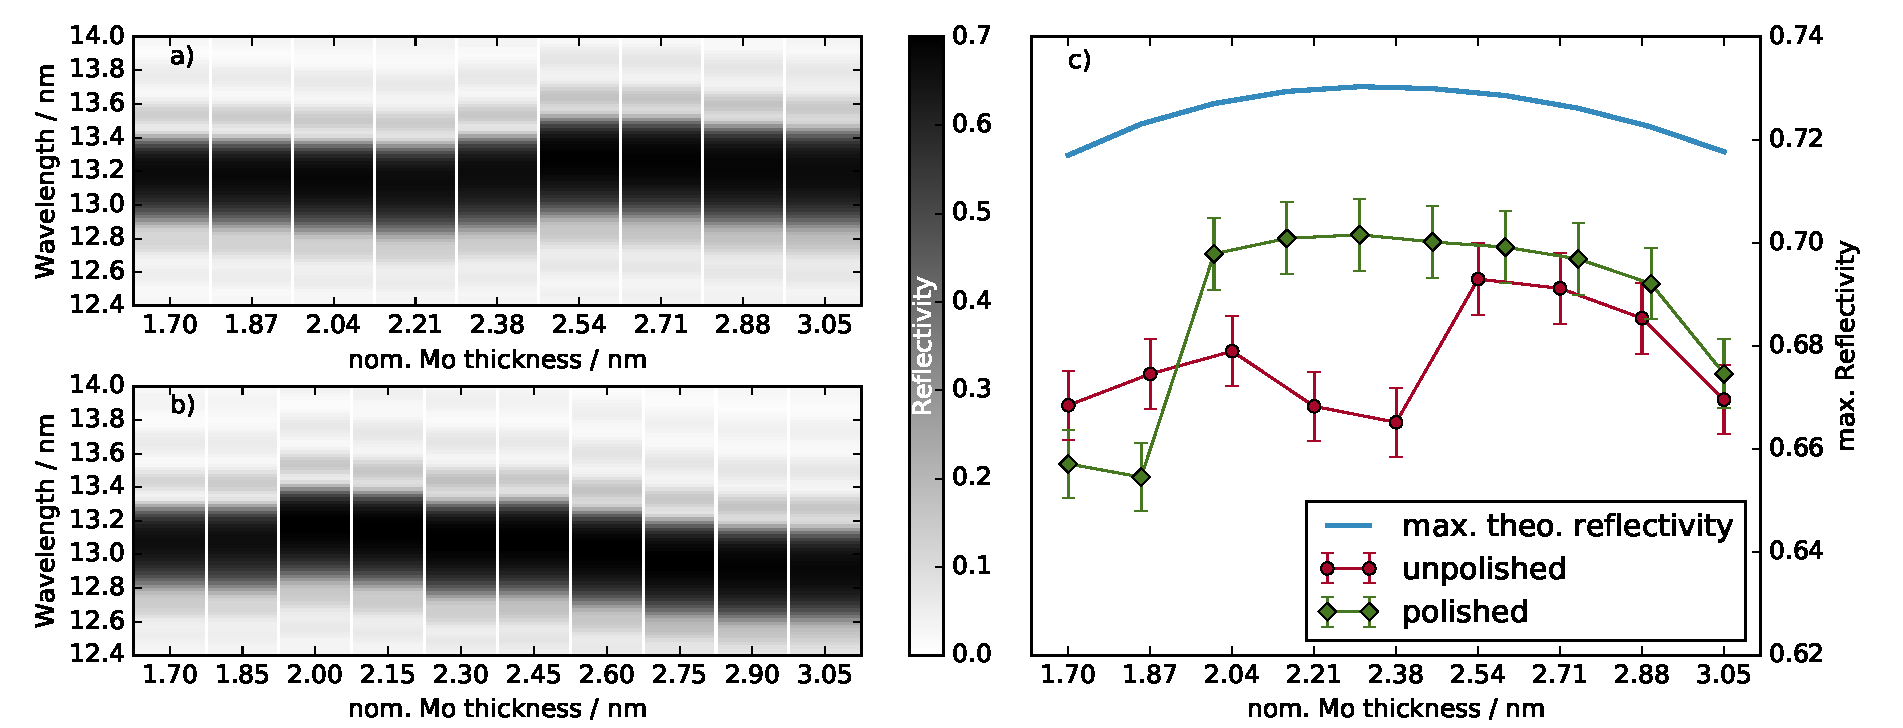
\includegraphics[width=\textwidth]{images/EUV_reflectivity_with_peak}
\caption{a) Reflectivity curves for the unpolished samples across the wavelength at a fixed angle of incidence of $\alpha_i = 15^\circ$ from the surface normal. The nine samples differ by the nominal Mo layer thickness indicated at the bottom axis. b) Reflectivity curves of the ten polished samples measured under the same conditions as for the first sample set. c) Respective peak reflectance values for each sample obtained from the measurements in (a) and (b) in comparison. The maximum theoretical reflectance is shown for a perfect (no roughness or interdiffusion) layer system with the same specifications as the samples.}
\label{fig:EUV_reflectivity}
\end{figure*}
Clear shifts of central peak reflectance wavelength can be observed in both cases. This coincides with a dip in the max.~peak reflectance in both cases, which most likely is associated with the crystallization threshold of the Mo layer. There is a notable difference in the observed jumps for the two sample sets. For the unpolished samples, the crystallization threshold seems to be around $d^\text{nom}_\text{Mo} =2.38$ nm, whereas it appears at much lower nom. Mo thickness values for the polished sample set at around  $d^\text{nom}_\text{Mo} =2.00$ nm. For all of the samples additional XRR measurements exist (not shown here), which were analyzed based on the combined principle using the MCMC method as described in Sec.~\ref{sec:max_likelihood}. An unambiguous result was only found with respect to the thickness parameters of Mo and Si, as well as for the N\'{e}vot-Croce parameter $\sigma$, whereas all other parameters show equal likelihood within the predefined boundaries. Therefore, the best model was obtained in a two-step process. First an MCMC optimization was performed including all parameters. Proceeding from this, the value of the Mo thickness with its confidence interval was obtained by marginalizing over all other parameters. In a second step, another MCMC optimization was performed on a reduced parameter set, fixing the layer thicknesses of the C barrier layer and the MoSi$_2$ interdiffusion layer to their nominal values of $d_C = d_{\text{MoSi}_2} = 0.5 $ nm. Thereby, comparable models could be derived for all samples without constraining the applicability of the model with respect to the data available. This comes with no consequences for the goal of analyzing the at-wavelength diffuse scattering, since the relative thickness of the barrier layer and the intermixing layer has only negligible effect on the fields inside the stack if the model fits the EUV reflectivity curve in the same spectral range. It should be noted here that for an entirely unambiguous characterization more complementary characterization methods, such as resonant EUV reflectivity and X-ray standing wave analysis, would be required as described in~\cite{haase_multiparameter_2016}.

The results of the two-step analysis are shown in Fig.~\ref{fig:fitted_mo_and_fitted_D}.
\begin{figure*}[htbp]
\centering
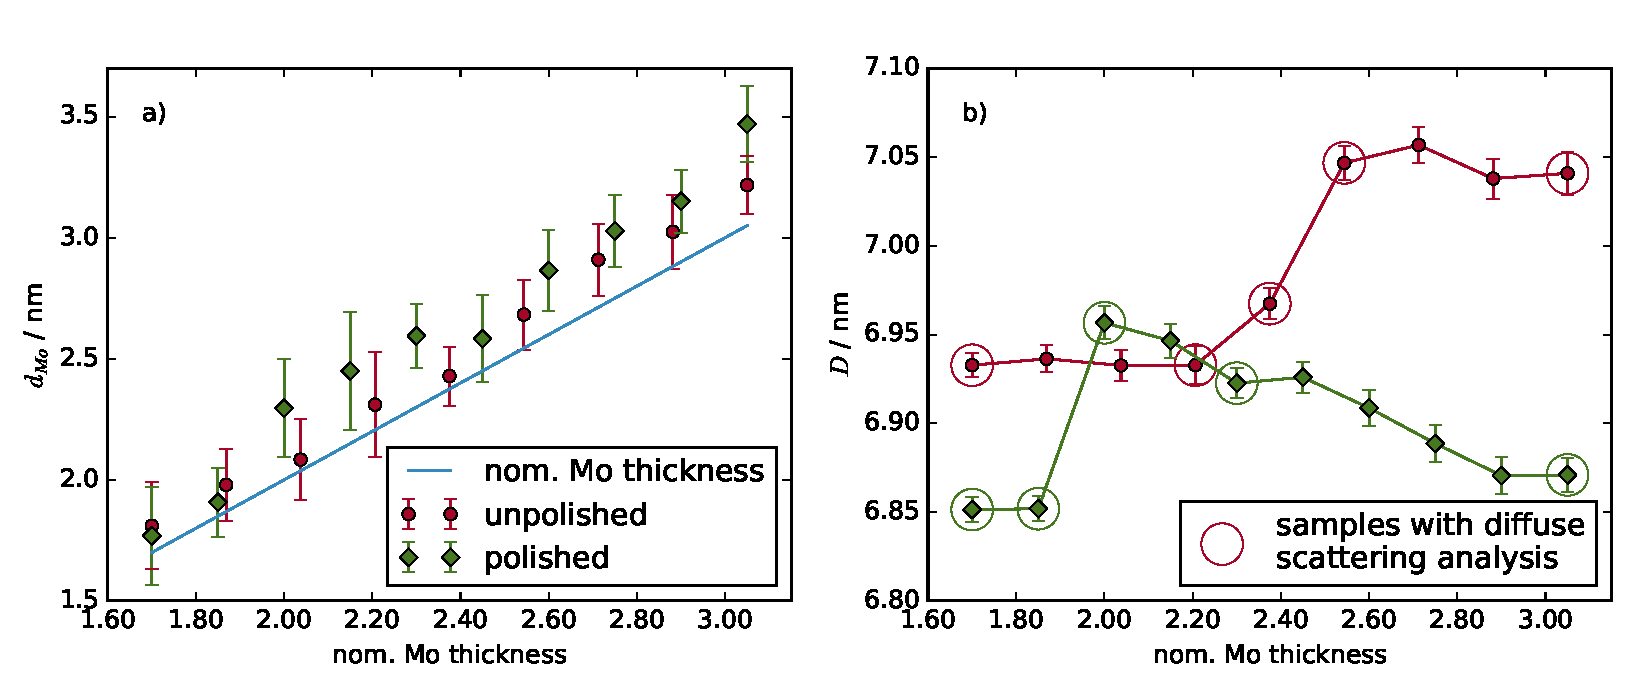
\includegraphics[width=\textwidth]{images/fitted_mo_and_fitted_D}
\caption{a) Fitted Mo thickness values for both sample sets resulting from the MCMC analysis (see text). The nominal Mo layer thickness is shown in comparison in good agreement with the obtained thicknesses. b) Fitted total period thickness $D$ for both sample sets. For both sample sets, clear jumps can be observed at approx.~$d^\text{nom}_\text{Mo} =2.00$ nm and $d^\text{nom}_\text{Mo} =2.38$ nm, respectively, which is attributed to the crystallization threshold (see text). The marked (circle) samples were measured and analyzed with respect to the diffuse scattering.}
\label{fig:fitted_mo_and_fitted_D}
\end{figure*}
The confidence intervals shown in Fig.~\ref{fig:fitted_mo_and_fitted_D}a are one standard deviation of the likelihood determined for the Mo layer thickness by the first-step MCMC procedure. The results show good agreement with the nominal thicknesses for both sample sets. The corresponding total period thicknesses $D$ in Fig.~\ref{fig:fitted_mo_and_fitted_D}b show clear jumps correlated with the presumed crystallization thresholds inferred from the max.~peak reflectivity in Fig.~\ref{fig:EUV_reflectivity}c. The results from this layer thickness and density characterization form the basis for the following analysis of the diffuse scattering.

\subsection{Obervation of the Crystallization Threshold}


\section{Analysis of Cr/Sc Multilayers with Sub-nanometer Layer Thickness}

\subsection{Reconstruction with a Binary Model Approach}
To better illustrate the requirement of an improved model, we have conducted an 
analysis based on the standard binary model of a Cr/Sc multilayer. The analysis 
was done based on the EUV data shown in Fig.~\ref{fig:EUV_XRR_REUV_XRF_data}a. 
The results are shown in Fig.~\ref{fig:EUV_XRR_reflectance} in comparison with 
the expected XRR curve from this optimization result and the theoretically 
achievable maximum reflectance without any roughness or interdiffusion. The Sc 
to Cr ratio was found to be $\Gamma_\text{Sc}=0.48$ with roughness and 
interdiffusion considered via a Nevot-Croce factor using $\sigma=0.385$ nm. The 
individual layer thicknesses for this sample were fitted to be $d_\text{Cr} = 
0.81$ nm and $d_\text{Sc}= 0.75$ nm. While the EUV reflectance curve (cf.~inset 
in Fig.~\ref{fig:EUV_XRR_reflectance}) shows excellent agreement with the 
measured data, there is a significant offset in the case of the XRR measurement 
with the (binary) model derived from the EUV reflectance experiment. Even a 
combined analysis could not yield a consistent result, since the Nevot-Croce 
factor required to reduce the theoretical EUV reflectance down to the measured 
level could not be brought into agreement with the XRR curve (result not shown 
here). In a strictly binary model with a layer thickness ratio of 
$\Gamma_\text{Sc}\approx 0.5$, the second Bragg peak is additionally suppressed 
due to symmetry reasons. Thus, there is a clear mismatch with the experimental 
observation as seen in the comparison of the fitted and measured XRR curves in 
Fig.~\ref{fig:EUV_XRR_reflectance}.
\begin{figure*}[htbp]
  \centering
  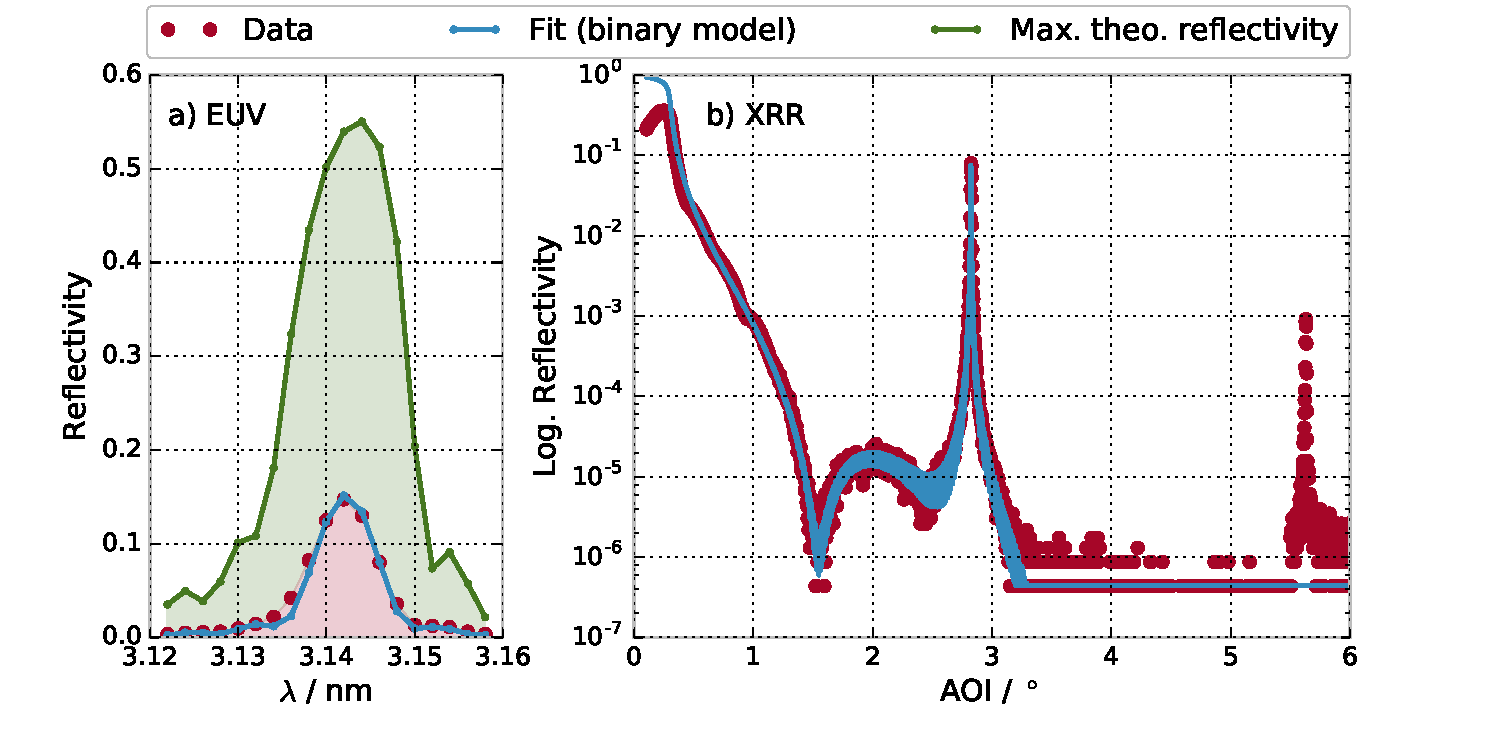
\includegraphics[width=\textwidth]{images/binary_model_and_theo_refl}
  \caption{a) Fitted experimental EUV reflectance curves across the wavelength 
of the radiation impinging at $1.5^\circ$ from normal, based on the binary 
model. The green curve shows the maximum possible reflectance in the water 
window assuming a perfect multilayer system without roughness or 
interdiffusion. b) The optimal model based on the analysis of the EUV 
reflectance (cf.~Fig.~\ref{fig:EUV_XRR_reflectance}a) shows a clear mismatch 
with the measured XRR curve in the second Bragg peak.
}
  \label{fig:EUV_XRR_reflectance}
\end{figure*}

\subsection{Extending The Model to Graded Interfaces and Interdiffusion}
Instead of the simple binary layer model, a gradual interface model is 
introduced to better reflect the electron density profile due to 
interdiffusion. A corresponding profile is shown in Fig.~\ref{fig:CrScModel} 
for illustration in comparison to the binary model.
\begin{figure*}[htbp]
  \centering
  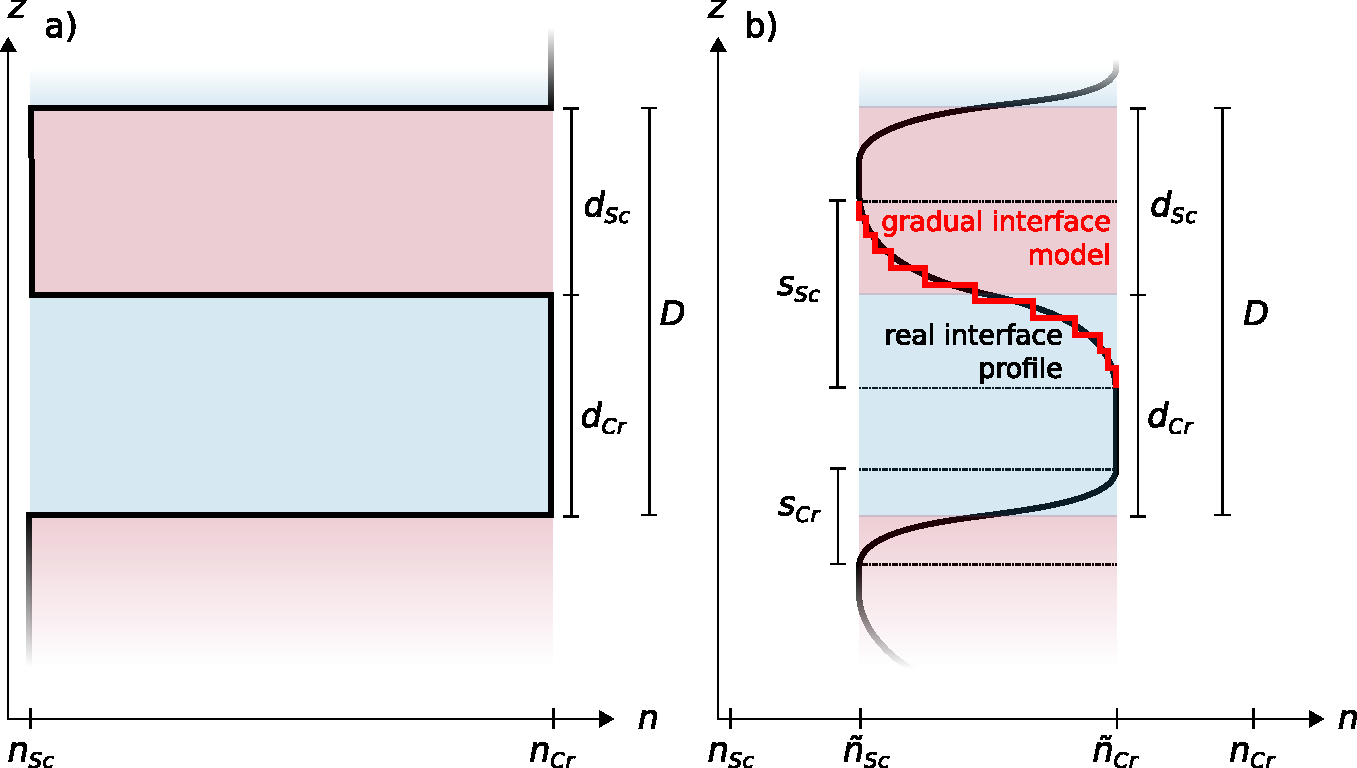
\includegraphics[width=\textwidth]{images/CrSc_model}
  \caption{a) Binary Cr/Sc multilayer model with total period thickness $D$ and 
the individual layer thicknesses $d_\text{Sc}$ and $d_\text{Cr}$. b) Model with 
explicit gradual interfaces following a sinusoidal profile. The ideal interface 
profile is approximated through discrete sublayers as indicated in red, forming 
the actual gradual interface profile entering the electric field calculations. 
The thickness of the interdiffusion zones can differ for the top and bottom 
interface in each period. Their total thicknesses are given by $s_\text{Sc}$ 
and $s_\text{Cr}$. The effective index of refraction for both layers is given 
by $\tilde{n}_\text{Sc}$ and $\tilde{n}_\text{Cr}$, respectively.}
  \label{fig:CrScModel}
\end{figure*}
The calculation of the electromagnetic fields is then conducted based on this 
model with the matrix formalism introduced in the preceding section. The 
interface region with sinusoidal profiles is sampled with a fixed number of 
equally spaced points in $z$-direction, effectively creating a region of thin 
sublayers with a gradually changing index of refraction. The parameters of our 
multilayer model are listed in Table~\ref{tbl:parametrization},
\begin{table*}
\centering
\caption{Multilayer parametrization and parameter limits}
\label{tbl:parametrization}
\begin{tabular}{@{}llll@{}}
\toprule
Parameter & Definition & Lower bound & Upper bound\\ \midrule
$D$ / nm & $= d_\text{Sc} + d_\text{Cr}$ & 1.5&1.6 \\ 
$\Gamma_{Sc}$ & $= d_\text{Sc} / D$&0.0 &1.0 \\ 
$s_d$ / nm&$=s_\text{Sc} + s_\text{Cr}$&0.0 & 1.6\\ 
$\Gamma_s$ &$= s_\text{Sc} / s_d$& 0.0& 1.0\\ 
$\eta$ &layer intermixing& 0.0& 1.0\\ 
$\sigma_r$ / nm & r.m.s.~roughness& 0.0& 0.5\\ 
$\rho_{Sc}$ &Sc density w.r.t.~bulk density & 0.5& 1.0\\ 
$\rho_{Cr}$ &Cr density w.r.t.~bulk density& 0.5& 1.0\\ 
 \bottomrule
\end{tabular}
\end{table*}
where $D$ is the full period thickness, $d_\text{Sc}$ and $d_\text{Cr}$ are the 
nominal layer thicknesses of the Cr and Sc layers as indicated in 
Fig.~\ref{fig:CrScModel}, and $\rho_\text{Sc}$ and $\rho_\text{Cr}$ their 
respective densities with respect to their bulk densities 
$\tilde{\rho_\text{Sc}} = 2.989$ g/cm$^3$ and $\tilde{\rho_\text{Cr}} = 7.19$ 
g/cm$^3$ \cite{henke_x-ray_1993}. The parameters $s_\text{Sc}$ and $s_\text{Cr}$ describe 
the full width of the interdiffusion layers as shown in 
Fig.~\ref{fig:CrScModel}. To take into account intermixing extending across the 
full period, we introduced an intermixing parameter $\eta$. The effective 
indices of refraction of the individual Cr and Sc layers are then given through
\begin{align}
\tilde{n}_\text{Cr} &=(\eta/2) n_\text{Sc} + (1-\eta/2) n_\text{Cr} \text{,} 
\nonumber\\
\tilde{n}_\text{Sc} &=(1-\eta/2) n_\text{Sc} + (\eta/2) n_\text{Cr} \text{,} 
\label{eqn:effective_n} \\
&\text{for} \quad \eta \in [0,1] \text{,}\nonumber
\end{align}
where $n_\text{Cr}$ and $n_\text{Sc}$ are the tabulated values \cite{henke_x-ray_1993} 
with densities $\rho_\text{Cr}$ and $\rho_\text{Sc}$. The loss of specular 
reflectance due to roughness-induced scattering is considered through the 
Nevot-Croce factor using $\sigma_\text{r}$ identical at each interface for the 
reasons described in the above section. To improve the optimization procedure 
and to reduce correlations between individual parameters, we have selected some 
effective parameters as defined in Table~\ref{tbl:parametrization}. The 
parameter $\Gamma_\text{Sc}$ indicates the portion of the Sc layer thickness 
with respect to the full period thickness $D$; $\Gamma_\sigma$ describes the 
asymmetry of the widths of the sinusoidal profiles at the Cr/Sc and Sc/Cr 
interfaces and is limited to the interval $\Gamma_\sigma \in [0,1]$. Note that 
$s_\text{Sc}$ and $s_\text{Cr}$ are half periods of the sinus functions used to 
describe the interface profiles. Therefore the condition $s_\text{Sc} + 
s_\text{Cr} \leq D$ holds.

\subsection{Combination of Complementary Experimental Methods}
The reconstruction of the multilayer structure was conducted with a series of 
experiments. The minimization functional of the combined analysis of the 
optimization problem $\chi^2$ is defined as the total sum of the reduced 
least-squares functionals for each experiment,
\begin{align}
\chi^2 = \tilde{\chi}^2_\text{EUV} +\tilde{\chi}^2_\text{XRR} 
+\tilde{\chi}^2_\text{REUV} + 
\tilde{\chi}^2_\text{GIXRF(Sc)}+\tilde{\chi}^2_\text{GIXRF(Cr)}\text{,} 
\label{eqn:total_chi_2}
\end{align}
where each of the reduced functionals is defined as
\begin{align}
\tilde{\chi}^2 = \frac{1}{m - p} \bigg[\sum\limits_{m} \frac{(I_m^\text{model} 
- I_m^\text{meas})^2}{\tilde{\sigma}_m^2} \bigg] \text{,} 
\label{eqn:reduced_chi_2}
\end{align}
with $m$ being the number of measurement points in each experiment and $p$ the 
number of parameters for the model. Statistical and systematic uncertainties 
for each data point are included in $\tilde{\sigma}_m$. The definition of 
Eq.~\eqref{eqn:total_chi_2} ensures that all experiments are weighted equally 
considering their respective uncertainties.

The minimization is performed with a particle-swarm optimizer (PSO) 
\cite{kennedy_particle_2011}. In the case of an optimization problem with many local 
minima, this provides an advantage with respect to gradient methods, where the 
fit result is dependent on the choice of starting values. Similar approaches 
employing genetic algorithms for solving the inverse problem of scatterometry 
can be found in the literature \cite{del_rio_modeling_2000}. In the case of the model 
parametrization given in Sec.~\ref{sec:model}, the choice of the parameter 
intervals is defined either by physical plausibility or the fact that the 
parameter is intrinsically defined in a certain interval, the same as for the 
intermixing $\eta$, for example. The intervals used in our analysis are listed 
in Table \ref{tbl:parametrization}.

The PSO analysis was conducted for each experiment individually and for the 
combination of all experiments. In the case of the XRR measurements, only the 
first and second Bragg peaks were considered for the combined analysis. The 
region in between mainly reflects the top surface layers, i.e.~capping layers, 
and potential surface contamination layers, which were analyzed separately 
based exclusively on the XRR data. The results were added as fixed surface 
layers to the model for all theoretical calculations of all experiments. The 
analysis of the GIXRF experiment was conducted based on the fluorescence data 
at an excitation photon energy of $6.25$ keV for the Sc-K and Cr-K lines by spectral 
deconvolution using detector response functions.

\subsubsection{EUV and X-ray reflectivity}
\subsubsection{Resonant EUV Reflectivity}
\subsubsection{Grazing Incidence X-ray Fluorescence}

\subsection{Model Uniqueness and Confidence Intervals}
The solution of the inverse problem based on the particle swarm optimization 
technique ideally delivers the global minimum of the total $\chi^2$ functional 
in the specified parameter space. However, no information is obtained about the 
sensitivity of an experiment with respect to certain aspects of the model, 
i.e.~specific parameters. As an example one might consider the case of an EUV 
reflectance experiment, where the influence of the interdiffusion layer 
asymmetry on the expected reflectance curve is negligible. The model reflects 
this geometry through the parameter $\Gamma_\sigma$. Most likely, an optimal 
choice for $\Gamma_\sigma$ minimizing $\chi^2$ exists and can be found by using 
the particle swarm optimizer. Nevertheless, varying the parameter 
$\Gamma_\sigma$ causes only marginally larger $\chi^2$, resulting in a limited 
credibility and validity of this parameter and leaving it essentially undefined 
based on the available data. To solve this issue and quantify confidence 
intervals for each parameter in each experiment, we apply a Markov-chain Monte 
Carlo (MCMC) sampling technique. The likelihood of the model describing the 
actual sample based on the data available is given by
\begin{align}
\mathcal{L}(\vec{x}) \propto \exp \big(-\chi^2 / 2 \big) \text{,} 
\label{eqn:likelihood}
\end{align}
where $\vec{x}$ is the set of parameters of the model and $\chi^2$ is the total 
$\chi^2$ for the validation of the combined analysis 
(cf.~Eq.~\eqref{eqn:total_chi_2}) or the reduced $\tilde{\chi}^2$ for the 
validation of the individual experiments according to the definition in 
Eq.~\eqref{eqn:reduced_chi_2}.
We employ an existing Python-based implementation of this sampling technique 
\cite{foreman-mackey_emcee:_2013} to numerically sample the likelihood functional in 
Eq.~\eqref{eqn:likelihood}. As a starting point we use the optimum parameter 
set obtained as a result of the particle swarm optimization.

Consequently, in addition to fitting the data with a particle swarm optimizer, 
each result was verified based on the MCMC method described above to evaluate 
the confidence intervals for each parameter. The two step process, i.e.~the PSO 
fitting procedure followed by the MCMC sampling, was conducted for each 
standalone experiment as well as for the combined optimization problem stated 
in Eq.~\eqref{eqn:total_chi_2}. The results are compiled in Table 
\ref{tbl:results}. The confidence intervals were calculated by evaluating the 
probability distribution as a result of the MCMC procedure for each parameter 
around its PSO fit results. The confidence intervals given here represent 
percentiles of the number of samples found in the interval defined by the upper 
and lower bounds used for the PSO procedure for each parameter. In the case of 
a centered Gaussian distribution, percentiles of $2.3\%$ and $97.8\%$ of the 
integrated number of samples forming the distribution, mark the interval of 
four times the standard deviation, i.e.~$\pm 2\sigma$ in statistical terms. Due 
to potential asymmetries in the actual distributions found by the MCMC method, 
explicit upper and lower bounds of the confidence intervals are given in Table 
\ref{tbl:results} based on these percentiles. The best model value is based on 
the PSO fit result and is refined by the MCMC sampling by calculating the mean 
value, i.e.~the 50\% percentile, of the distribution of samples following the 
MCMC procedure. The best model is thus the result of a two-step optimization 
routine starting with a PSO analysis and sampling based on the resulting values 
to evaluate the distribution according to Eq.~\eqref{eqn:likelihood}.
\onecolumn
\begin{table*}
\centering
\caption{Optimized model parameters with confidence intervals derived from MCMC 
validation for each individual experiment and the combined analysis}
\label{tbl:results}
\begin{tabular}{@{}llllll@{}}
\toprule
Parameter &  Combined & EUV  & XRR  & REUV  & GIXRF\\ \midrule
$D$ / nm& $1.5737_{-0.0010}^{+0.0008}$ & $1.5749_{-0.0022}^{+0.0014}$ & 
$1.5726_{-0.0042}^{+0.0035}$& $1.5728_{-0.0019}^{+0.0016}$& 
$1.5741_{-0.0024}^{+0.0021}$ \\ \addlinespace
$\Gamma_{Sc}$ & $0.48_{-0.04}^{+0.04}$ & $0.35_{-0.11}^{+0.14}$ & 
$0.42_{-0.26}^{+0.35}$& $0.52_{-0.07}^{+0.09}$& $0.49_{-0.10}^{+0.09}$ \\ 
\addlinespace
$s_d$ / nm& $1.34_{-0.26}^{+0.18}$ & $0.72_{-0.66}^{+0.67}$ & 
$0.60_{-0.57}^{+0.78}$& $0.89_{-0.83}^{+0.59}$& $1.27_{-0.38}^{+0.24}$ \\ 
\addlinespace
$\Gamma_\sigma$ & $0.16_{-0.16}^{+0.51}$ & $0.29_{-0.28}^{+0.64}$ & 
$0.40_{-0.39}^{+0.57}$& $0.33_{-0.32}^{+0.61}$& $0.39_{-0.37}^{+0.57}$ \\ 
\addlinespace
$\eta$ & $0.56_{-0.16}^{+0.06}$ & $0.44_{-0.30}^{+0.16}$ & 
$0.38_{-0.36}^{+0.33}$& $0.52_{-0.37}^{+0.14}$& $0.37_{-0.34}^{+0.25}$ \\ 
\addlinespace
$\sigma_r$ / nm& $0.11_{-0.10}^{+0.11}$ & $0.17_{-0.15}^{+0.12}$ & 
$0.13_{-0.12}^{+0.14}$& $0.17_{-0.16}^{+0.16}$& $0.27_{-0.25}^{+0.20}$ \\ 
\addlinespace
$\rho_{Sc}$ & $0.94_{-0.12}^{+0.05}$ & $0.84_{-0.32}^{+0.15}$ & 
$0.78_{-0.27}^{+0.21}$& $0.94_{-0.14}^{+0.06}$& $0.83_{-0.30}^{+0.17}$ \\ 
\addlinespace
$\rho_{Cr}$ & $0.98_{-0.08}^{+0.02}$ & $0.96_{-0.13}^{+0.04}$ & 
$0.83_{-0.27}^{+0.16}$& $0.90_{-0.21}^{+0.09}$& $0.86_{-0.28}^{+0.14}$ \\ 
\addlinespace
 \bottomrule
\end{tabular}
\end{table*}
%\twocolumn
The confidence intervals of each experimental method differ significantly 
depending on the parameter. To better demonstrate the different sensitivities 
for the model parameters depending on the experimental method, we have 
illustrated each confidence interval in Fig.~\ref{fig:confidence_intervals}.
\begin{figure}[htbp]
  \centering
  
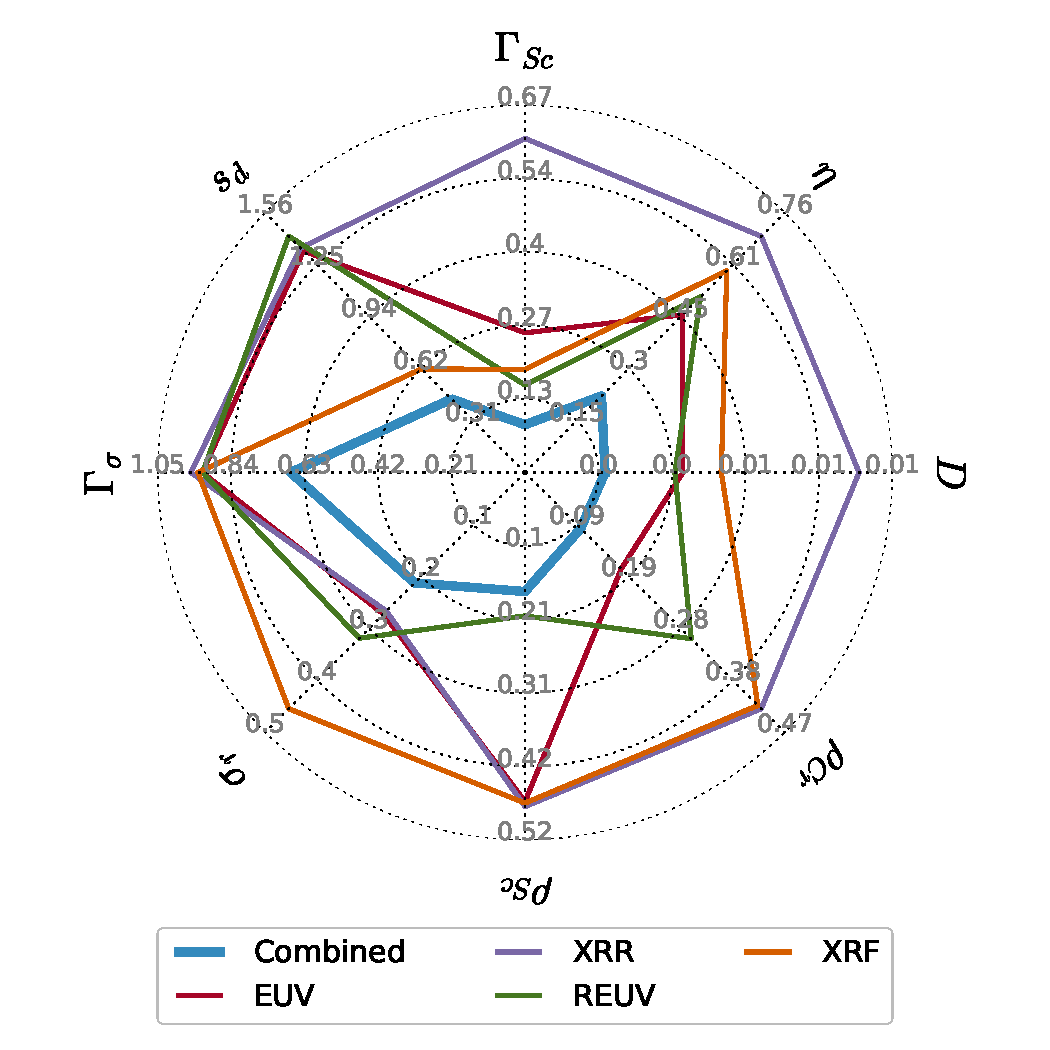
\includegraphics[width=0.6\textwidth]{images/spiderplot_confidence_intervals_empty}
  \caption{Visual representation of the total confidence intervals for each of 
the parameters with respect to each of the individual experiments as well as 
the combined analysis.}
  \label{fig:confidence_intervals}
\end{figure}
It is worth noting that the confidence interval for the combined analysis is 
significantly smaller compared to the individual experiments. This is 
especially true for the parameter $\Gamma_\sigma$ describing the asymmetry of 
the interdiffusion layers. Within each of the individual experiments this 
parameter has a large uncertainty, whereas the combined analysis delivers a 
significant result of a clearly asymmetric interdiffusion layer thickness.


%\section{Results and Discussion} \label{sec:results}

The best fit result based on the two-step optimization procedure of the 
combined data set of all experiments is shown in 
Fig.~\ref{fig:combined_fit_result} together with the experimental data. The 
theoretical calculations based on the above model and the experimental data 
show good agreement. Nevertheless, differences can be observed. The reason lies 
in the fact that the model is potentially still too ideal. Small variations 
during the deposition process, for example, could lead to imperfections, which 
are not described in a strictly periodic model. However, including these by 
explicitly breaking the periodicity would again lead to an ill-defined model 
with a vastly increased number of parameters and is thus not practical. Another 
reason is the deviation in the homogeneity of the sample, e.g.~a varying period 
across the sample, which cause mismatches if the measurement position varies 
slightly between the different experimental setups. The latter effects were 
considered in the uncertainties of the individual measurements by measuring the 
EUV reflectivity at positions $\pm 2$ mm from the center position and fitting 
the model. The result was a $\Delta D = 2$ pm shift in the period over $4$ mm 
across the sample.
\onecolumn
\begin{figure*}[htbp]
  \centering
  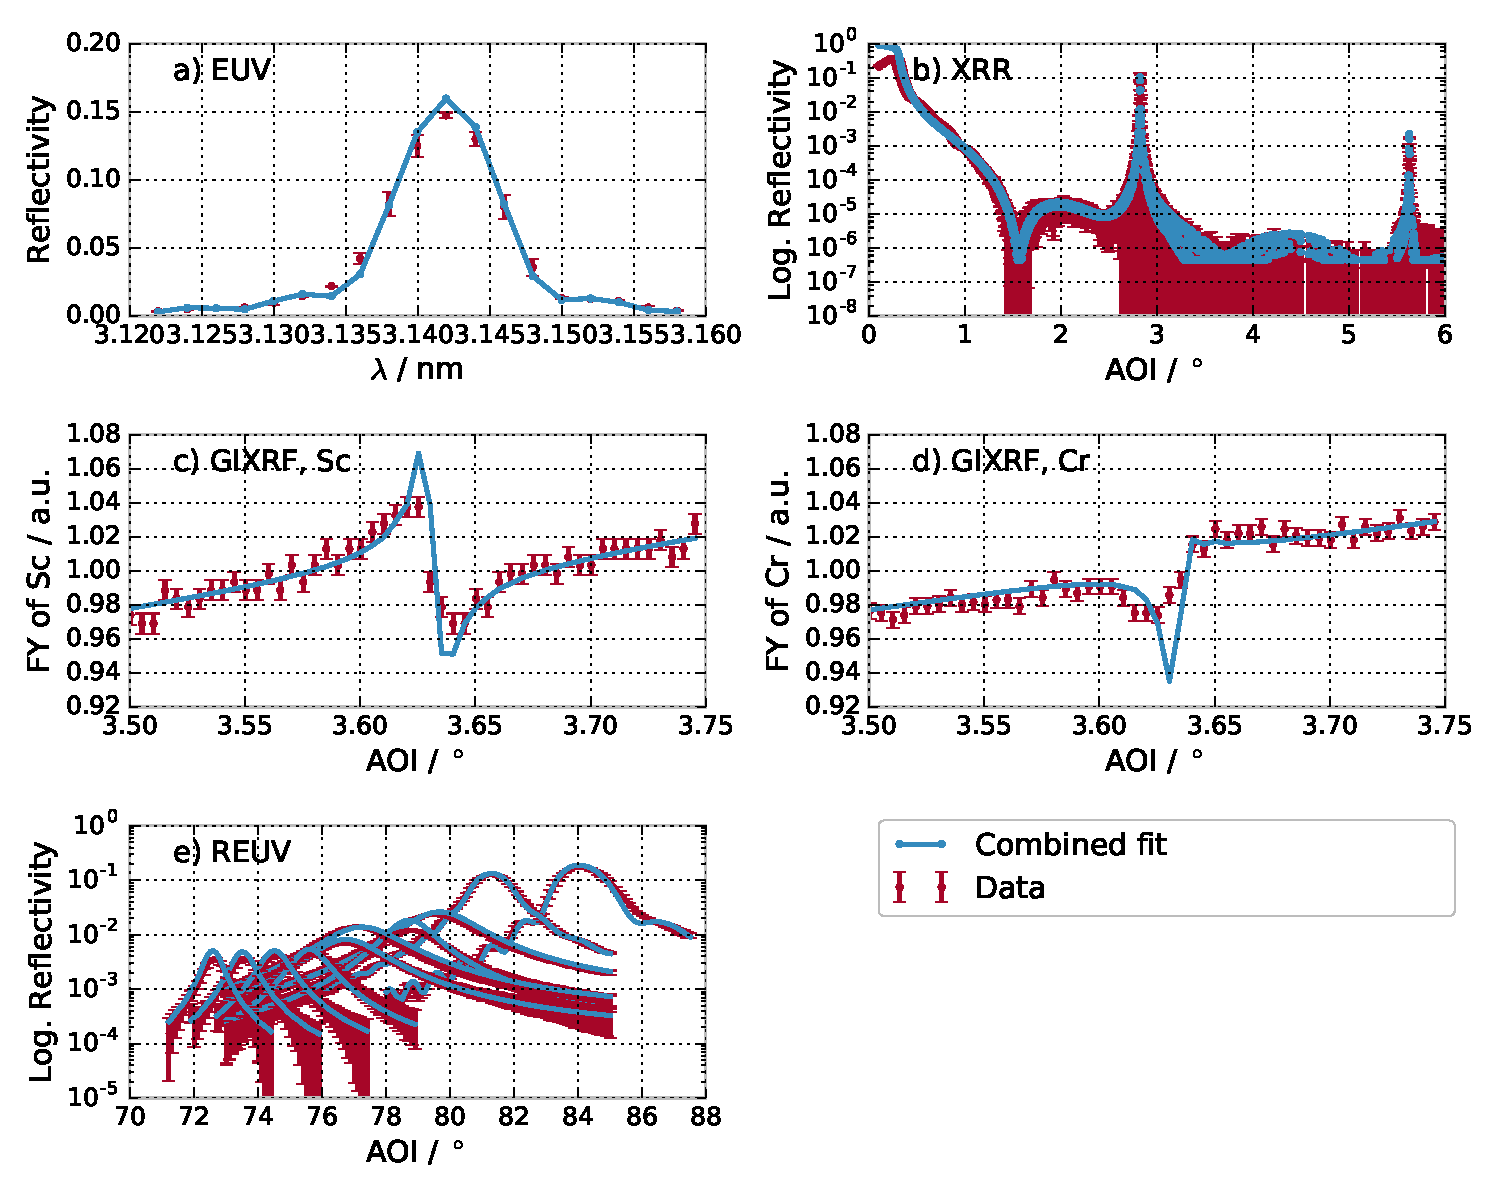
\includegraphics[width=\textwidth]{images/combined_fit_result}
  \caption{Measured and calculated reflectance and intensity curves for the 
optimized parameters with the combined analysis of all experiments as listed in 
Table~\ref{tbl:parametrization}.}
  \label{fig:combined_fit_result}
\end{figure*}
%\twocolumn
The resulting depth dependence of the index of refraction is shown in 
Fig.~\ref{fig:electron_density_profile} together with the initial binary model 
for comparison.
\begin{figure}[htbp]
  \centering
  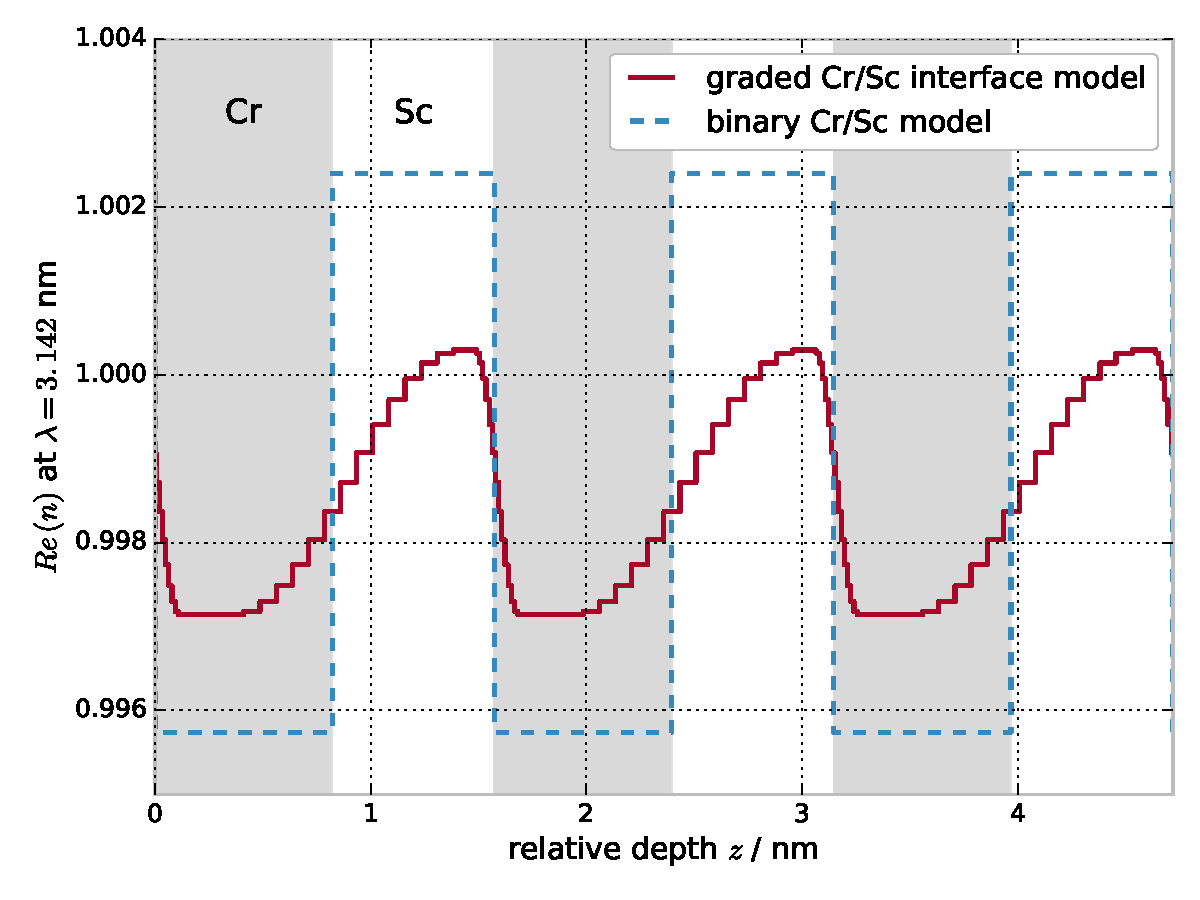
\includegraphics[width=0.7\textwidth]{images/real_model}
  \caption{Real part of the index of refraction $n$  based on the results of 
the optimized parameters listed in Table~\ref{tbl:results} for the combined 
analysis for a selected wavelength. The gradual interface model is shown in 
direct comparison to the binary model optimized for the EUV reflectance curve 
over three full periods. The resulting strong asymmetry in the width of the 
interface regions is clearly visible (see text). The gray and white shaded 
areas indicate the Cr and Sc layers, respectively, for the binary model.}
  \label{fig:electron_density_profile}
\end{figure}
The most remarkable result of the combined analysis is the strong asymmetry of 
the interdiffusion layers. This can only be shown by the combination of all 
analytical experiments conducted here, as can be seen from the confidence 
intervals in Fig.~\ref{fig:confidence_intervals} as well as the values in 
Table~\ref{tbl:results}. A possible explanation for this asymmetry is the 
deposition process through magnetron sputtering. The elements Cr and Sc have 
different mass and thus different momentum when deposited onto each other. A 
similar effect is known from the deposition of Mo/Si multilayer systems, where 
the heavier Mo shows higher penetration into the Si layer than vice versa 
\cite{petford-long_highresolution_1987}. In the case of Cr/Sc multilayers, the Cr is heavier and 
thus has higher momentum leading to a broader interdiffusion layer.
The validation using the MCMC procedure also yields possible correlations 
between single parameters of the model.

\cite{haase_multiparameter_2016}


